\subsection{T4: State Compression and Structural Aggregation}
\label{sec:t4}

\subsubsection{Family Overview and Meta-Pipeline Position}
\label{sec:t4-overview}

T4 contains optimizers whose primary contribution is to reduce the memory
footprint, granularity, precision, or lifetime of optimizer state.  For a
model with $d$ trainable parameters, AdamW stores at least two full-size state
tensors, $m_t$ and $v_t$, in addition to parameters, gradients, activations,
and distributed-training buffers.  This cost is significant in
LLM training, because optimizer state competes directly with model size, sequence
length, batch size, activation rematerialization, sharding, and communication
buffers.  The central
issue is which optimizer histories must be retained, how faithfully they must be
represented, and when they can be reconstructed, broadcast, dequantized, or
discarded.

\begin{figure}[t]
  \centering
  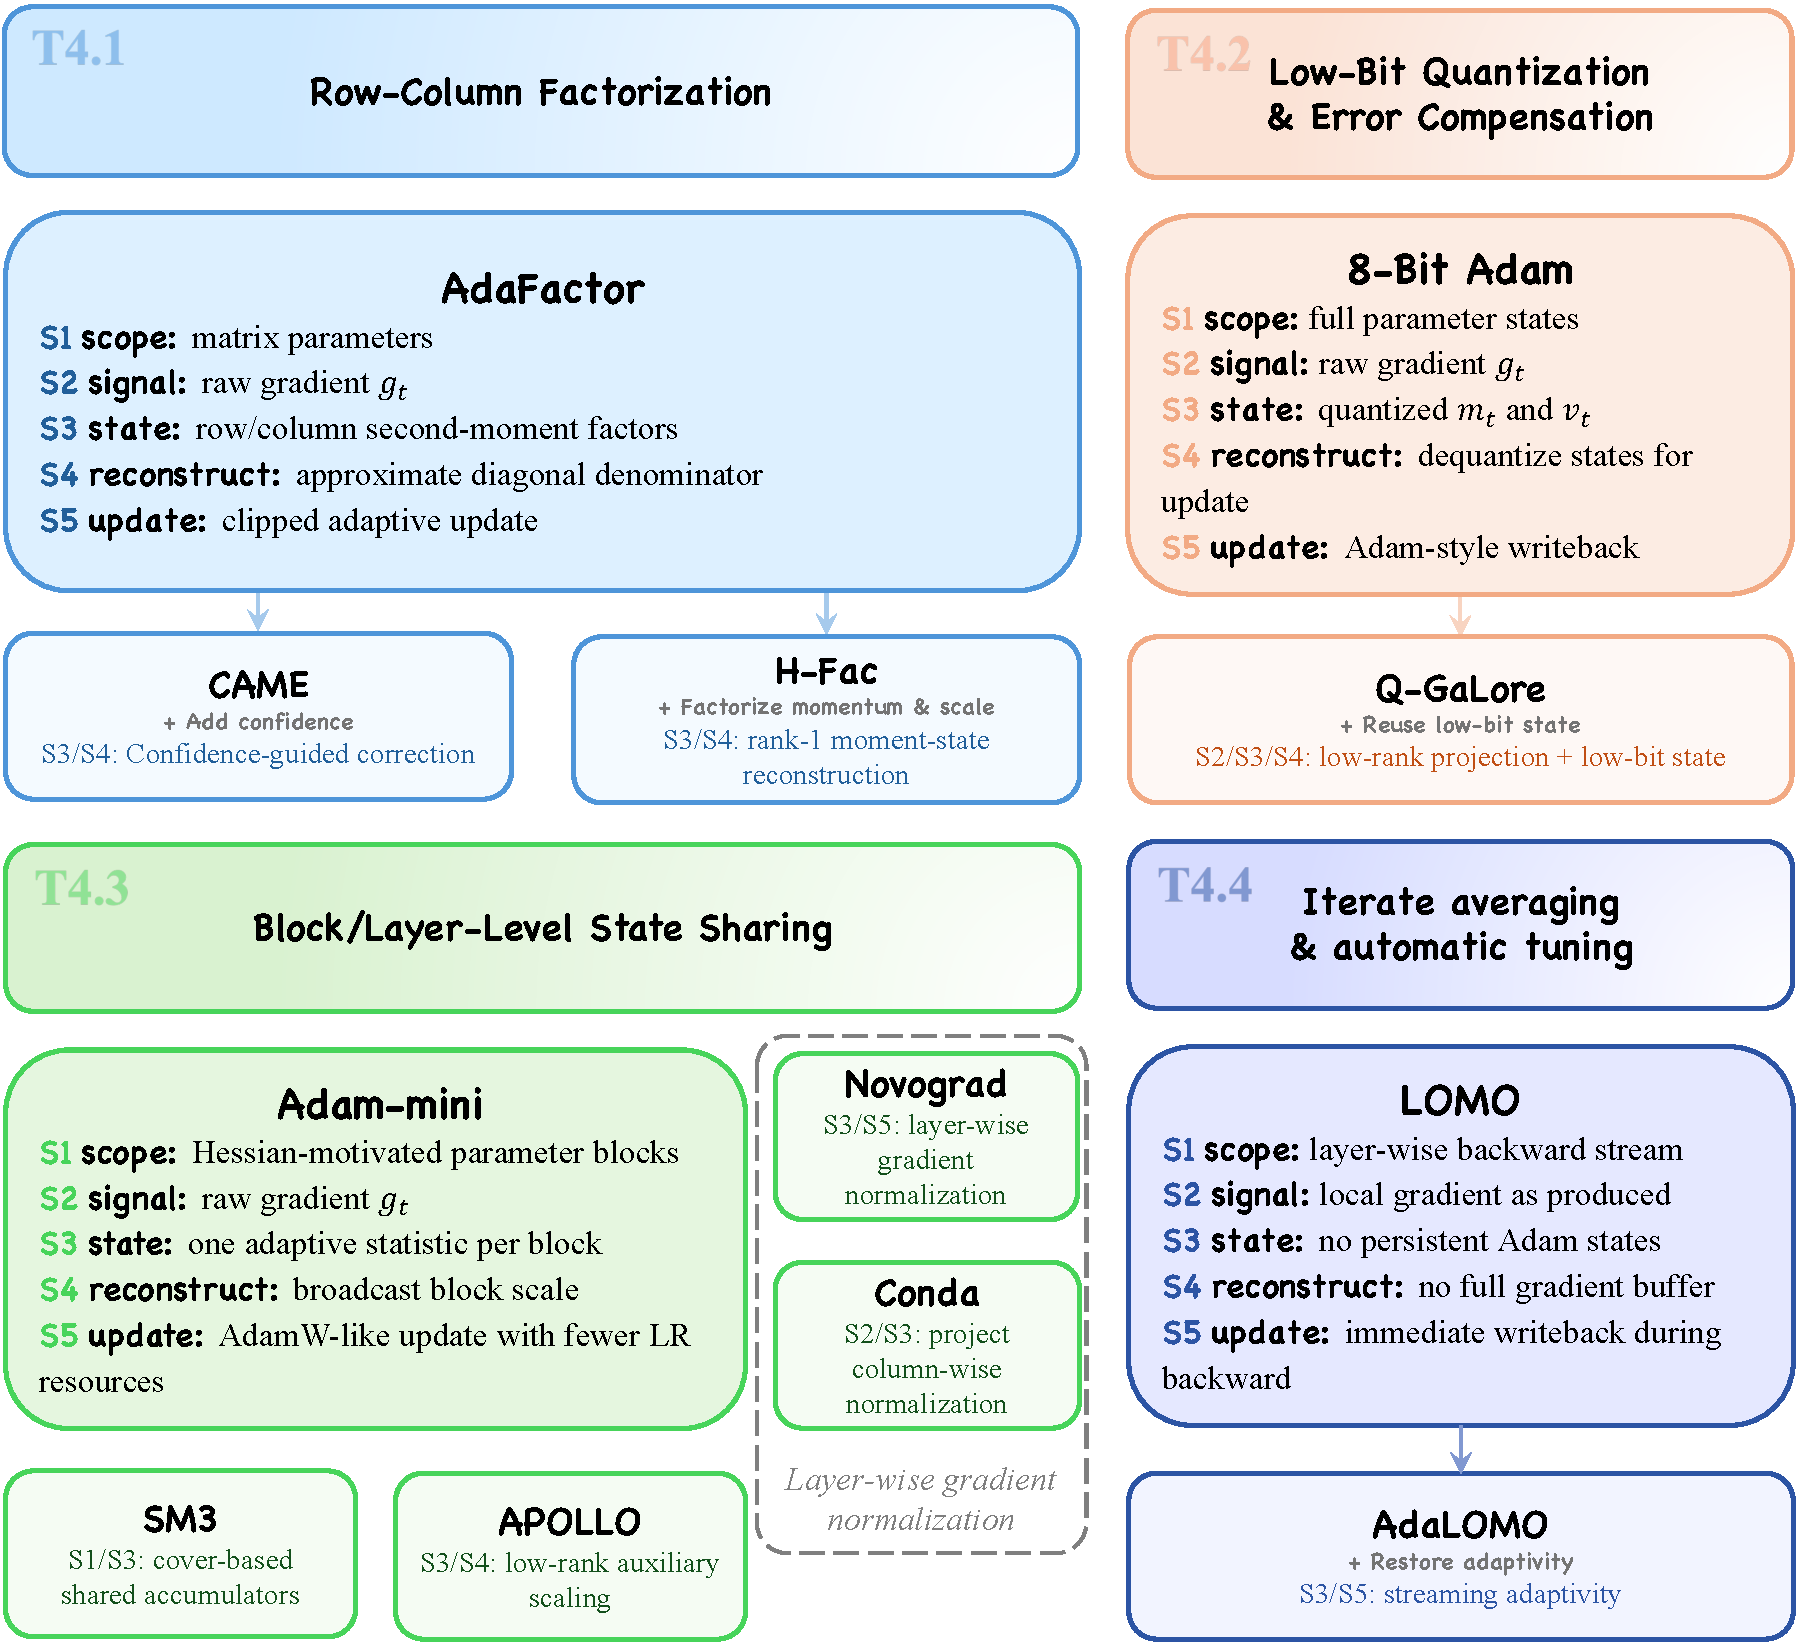
\includegraphics[width=0.75\linewidth]{figures/opt_t4.pdf}
  \caption{\textbf{Mechanism schematic for T4 state compression and structural
aggregation.} The schematic organizes the family by the form of memory
reduction: factored second-moment storage, low-bit state representation,
shared adaptive statistics, and streaming gradient consumption.}
  \label{fig:t4_family_mechanism}
\end{figure}

\paragraph{Subclass structure and membership.}
Figure~\ref{tab:t4_family_taxonomy} gives the subclass-level optimizer list for T4, and the
four subclasses below specify the corresponding optimizer membership.  The
split follows the state representation being changed.
\begin{enumerate}[label=\textbf{T4.\arabic*},leftmargin=*,itemsep=2pt]
  \item \textbf{Row-column factorization.}
  This subclass contains AdaFactor and CAME.  Its members replace a full
  matrix second-moment tensor with row and column summaries, then reconstruct
  an approximate denominator only when the update is formed
  ~\citep{shazeer2018adafactor,luo2023came}.
  \item \textbf{Low-bit quantization and error compensation.}
  This subclass contains 8-bit Adam and Q-GaLore.  Its members store optimizer
  statistics, projection objects, or related accumulated information in
  low-bit form and rely on block-wise scaling, stochastic rounding, or
  compensation logic to control long-horizon numerical error
  ~\citep{dettmers20218,zhang2024q}.
  \item \textbf{Block- and layer-level state sharing.}
  This subclass contains Adam-mini, APOLLO, SM3, Conda, and NovoGrad.  Its
  members reduce the number or dimensionality of adaptive statistics by
  sharing them across blocks, covers, columns, layers, or low-rank auxiliary
  structures~\citep{zhang2025adam,zhu2025apollo,anil2019memory,wang2025conda,ginsburg2019stochastic}.
  \item \textbf{Fused backprop-update.}
  This subclass contains LOMO and AdaLOMO.  Its members change the optimizer
  pipeline so that gradients are consumed during backpropagation as soon as
  they are produced
  ~\citep{lv2024full,lv2024adalomo}.
\end{enumerate}

At the family level, a compressed-state adaptive update can be summarized as
\begin{equation}
  \mathcal{Z}_t = \mathcal{C}_t(\mathcal{S}_t),\quad
  \widehat{\mathcal{S}}_t = \mathcal{R}_t(\mathcal{Z}_t),\quad
  \theta_{t+1}
  =
  \theta_t-\eta_t\,
  \mathcal{U}_t\big(g_t,\widehat{\mathcal{S}}_t\big),
  \label{eq:t4-state-compression-template}
\end{equation}
where $\mathcal{S}_t$ denotes the full optimizer state that an AdamW-like
method would store, $\mathcal{C}_t$ is a compression, sharing, quantization,
or lifetime-shortening map, $\mathcal{R}_t$ reconstructs or exposes the
usable state at update time, and $\mathcal{U}_t$ is the base update rule.
Full-state AdamW is the special case in which $\mathcal{C}_t$ and
$\mathcal{R}_t$ are identities.  T4 begins when at least one of them is
nontrivial.

In the meta-pipeline, T4 primarily modifies S3 and S4.  The state maintained
by S3 may be factored, quantized, shared, reduced to a low-dimensional
auxiliary object, or eliminated.  S4 then reconstructs, broadcasts,
dequantizes, or streams the required quantity into the update.  T4.3 also
uses S1 because the grouping of parameters into blocks, covers, columns, or
layers determines which coordinates share statistics.  T4.4 changes S5 as
well because the writeback occurs during the backward pass, before
all gradients have been materialized.

This definition separates T4 from nearby families.  GaLore belongs to T2.3
because it changes the mathematical subspace in which gradients and Adam
states are updated.  Q-GaLore is discussed in T4.2 only for the additional
quantization component on top of that low-rank mechanism
~\citep{zhao2024galore,zhang2024q}.  Lion uses less memory than AdamW,
but its primary mechanism is a sign-direction map, so it remains T3.  ZeRO,
activation checkpointing, CPU/NVMe offloading, and parameter-efficient
fine-tuning can be combined with T4 optimizers, but they are systems or
training-regime techniques in this taxonomy.  T4 is reserved for methods that change the optimizer's own state
representation or gradient-consumption pipeline.


% Auto-generated by code/generate_taxonomy_figures.py; do not edit by hand.
% \begin{table*}[!htbp]
%   \centering
%   \caption{Taxonomy of state-compressed and structurally aggregated optimizers.}
%   \label{tab:t4_family_taxonomy}
%   \scriptsize
%   \setlength{\tabcolsep}{4pt}
%   \renewcommand{\arraystretch}{1.16}
%   \arrayrulecolor{optHiddenBlack}
%   \begin{tabularx}{0.82\textwidth}{@{}>{\raggedright\arraybackslash}p{0.27\textwidth}>{\raggedright\arraybackslash}X@{}}
%     \hline
%     \textbf{Subclass} & \textbf{Optimizers} \\
%     \hline
%     \textbf{\textit{T4.1: Row-Column Factorization}} & AdaFactor~\cite{shazeer2018adafactor}, CAME~\cite{luo2023came} \\
%     \hline
%     \textbf{\textit{T4.2: Low-Bit Quantization \& Error Compensation}} & 8-bit Adam~\cite{dettmers20218}, Q-GaLore~\cite{zhang2024q} \\
%     \hline
%     \textbf{\textit{T4.3: Block/Layer-Level State Sharing}} & Adam-mini~\cite{zhang2025adam}, APOLLO~\cite{zhu2025apollo}, SM3~\cite{anil2019memory}, Conda~\cite{wang2025conda}, NovoGrad~\cite{ginsburg2019stochastic} \\
%     \hline
%     \textbf{\textit{T4.4: Fused Backprop-Update}} & LOMO~\cite{lv2024full}, AdaLOMO~\cite{lv2024adalomo} \\
%     \hline
%   \end{tabularx}
% \end{table*}

\definecolor{hidden-blue}{HTML}{4a90e2}
\definecolor{hidden-black}{HTML}{333333}
\tikzstyle{my-box}=[
  rectangle,
  draw=hidden-black,
  rounded corners,
  text opacity=1,
  minimum height=1.5em,
  minimum width=5em,
  inner sep=2pt,
  align=center,
  fill opacity=.5,
]
\tikzstyle{root}=[
  align=center,
]
\tikzstyle{leaf}=[
  my-box,
  minimum height=1.5em,
  text=black,
  font=\normalsize,
  inner xsep=5pt,
  inner ysep=4pt,
  text width=10.5em,
  fill opacity=1,
]
\tikzstyle{leaf1}=[
  my-box,
  minimum height=1.5em,
  fill=yellow!32,
  text=black,
  font=\normalsize,
  inner xsep=5pt,
  inner ysep=4pt,
  text width=17em,
  align=left,
]
\tikzstyle{leaf2}=[
  my-box,
  minimum height=1.5em,
  fill=hidden-blue!57,
  text=black,
  font=\normalsize,
  inner xsep=5pt,
  inner ysep=4pt,
  text width=17em,
  align=left,
]
\tikzstyle{leaf3}=[
  my-box,
  minimum height=1.5em,
  fill=purple!27,
  text=black,
  font=\normalsize,
  inner xsep=5pt,
  inner ysep=4pt,
  text width=17em,
  align=left,
]
\tikzstyle{leaf4}=[
  my-box,
  minimum height=1.5em,
  fill=teal!30,
  text=black,
  font=\normalsize,
  inner xsep=5pt,
  inner ysep=4pt,
  text width=17em,
  align=left,
]

\begin{figure*}[!htbp]
\centering
\resizebox{\textwidth}{!}{
\begin{forest}
forked edges,
for tree={
grow=east,
reversed=true,
anchor=base west,
parent anchor=east,
child anchor=west,
base=left,
font=\large,
rectangle,
draw=hidden-black,
rounded corners,
align=left,
minimum width=4em,
edge+={darkgray, line width=1pt},
s sep=4pt,
inner xsep=5pt,
inner ysep=4pt,
line width=1.1pt,
ver/.style={rotate=90, child anchor=north, parent anchor=south, anchor=center},
},
where level=1{text width=11em, font=\normalsize}{},
where level=2{text width=34.5em, align=left, tier=citations, font=\small}{},
[
    T4-based Optimizers,
    ver, fill=brown!10!white, text=hidden-black, root
    [
        T4.1: Row-Column Factorization,
        fill=yellow!32, leaf1
        [{
            AdaFactor~\cite{shazeer2018adafactor},
            CAME~\cite{luo2023came}
        }, fill=yellow!12]
    ]
    [
        T4.2: Low-Bit Quantization \& Error \\
        Compensation,
        fill=hidden-blue!57, leaf2
        [{
            8-bit Adam~\cite{dettmers20218},
            Q-GaLore~\cite{zhang2024q}
        }, fill=hidden-blue!15]
    ]
    [
        T4.3: Block/Layer-Level State \\ Sharing,
        fill=purple!27, leaf3
        [{
            Adam-mini~\cite{zhang2025adam},
            APOLLO~\cite{zhu2025apollo},
            BlockwiseLR~\cite{wang2025sharpness},
            Conda~\cite{wang2025conda},
            NovoGrad~\cite{ginsburg2019stochastic},\\
            SM3~\cite{anil2019memory},
            SAC~\cite{li2026sac},
            SGG~\cite{li2025taming}
        }, fill=purple!12]
    ]
    [
        T4.4: Fused Backprop-Update,
        fill=teal!30, leaf4
        [{
            LOMO~\cite{lv2024full},
            AdaLOMO~\cite{lv2024adalomo}
        }, fill=teal!12]
    ]
  ]
\end{forest}
}
\caption{Taxonomy of state-compressed and structurally aggregated optimizers.}
\label{tab:t4_family_taxonomy}
\end{figure*}

\subsubsection{LMO-Driven Four-Axis Interpretation}
\label{sec:t4-lmo-four-axis}

In the four-axis notation of Section~\ref{sec:lmo-four-axis}, T4 is the most
direct instantiation of state compression in Axis~II.  A generic adaptive update can be written as
\begin{equation}
  \theta_{t+1}
  =
  \theta_t
  - \eta_t\,
  \frac{\widehat{m}_t}{\sqrt{\mathcal{R}(\mathcal{C}(v_t))}+\epsilon},
  \label{eq:t4-compressed-denominator}
\end{equation}
where $\mathcal{C}$ compresses the second-moment state and $\mathcal{R}$
reconstructs, broadcasts, or dequantizes it for the update.  In full AdamW,
$\mathcal{C}$ and $\mathcal{R}$ are both identities.  In T4, at least one of
them is nontrivial.  The geometry of the base direction can remain
coordinate-wise Adam-like, and the innovation is the representation of the
statistics that control the denominator.

For matrix parameters $W_t\in\mathbb{R}^{m\times n}$, a factored method keeps
row and column statistics, for example
\begin{equation}
  r_{i,t}=\beta r_{i,t-1}+(1-\beta)\frac{1}{n}\sum_{j=1}^{n}G_{ij,t}^2,
  \quad
  c_{j,t}=\beta c_{j,t-1}+(1-\beta)\frac{1}{m}\sum_{i=1}^{m}G_{ij,t}^2,
  \label{eq:t4-row-column-states}
\end{equation}
and reconstructs an approximate matrix denominator such as
$\widehat{V}_{ij,t}\propto r_{i,t}c_{j,t}$.  This lowers state from
$O(mn)$ to $O(m+n)$, but it assumes that row and column summaries preserve
enough information about the diagonal curvature proxy.  For block sharing,
the compression map is instead a partition
$\{B_k\}_{k=1}^{K}$ with shared statistics
\begin{equation}
  s_{k,t} = \beta s_{k,t-1}
  +(1-\beta)\frac{1}{|B_k|}\sum_{i\in B_k}g_{i,t}^2,
  \quad i\in B_k,
  \label{eq:t4-block-sharing}
\end{equation}
which is then broadcast to all coordinates in the block.  The compression
quality depends on whether the partition aligns with the structure of the
loss landscape.

Low-bit methods preserve the same state shape but change the value
representation.  With a $b$-bit block quantizer $Q_b$, the stored state is
$Q_b(m_t)$ or $Q_b(v_t)$, and the update
uses $\operatorname{dequant}(Q_b(\cdot))$ at computation time.  The key design
choices are block size, dynamic range tracking, stochastic rounding, and
special handling of sensitive tensors such as embeddings.  Fused
backprop-update methods change a different part of Axis~II, namely that the state may not
be stored at all.  Gradients are consumed as soon as they are produced during
backpropagation, which changes the lifetime of $g_t$ and restricts operations
that require global gradient visibility.

\subsubsection{Representative Methods}
\label{sec:t4-methods}

\noindent
The following discussion follows the T4.1--T4.4 subclass order introduced
above.  Within each subclass, representative methods are grouped by the local
state operation they modify.

\paragraph{Row-Column Factorization.}
\label{sec:t4-factorized}

The first T4 branch replaces a dense matrix-valued second-moment state by two
marginal summaries.  For $G_t\in\mathbb{R}^{m\times n}$, the representative
template is
\begin{align}
  R_t &= \beta R_{t-1}+(1-\beta)\operatorname{rowmean}(G_t\odot G_t), \quad
  C_t = \beta C_{t-1}+(1-\beta)\operatorname{colmean}(G_t\odot G_t), \\
  \widehat{V}_{ij,t} &=\frac{R_{i,t}C_{j,t}}{\operatorname{mean}(R_t)},\quad
  \Delta_{ij,t}=\frac{\widehat{m}_{ij,t}}{\sqrt{\widehat{V}_{ij,t}}+\epsilon}.
  \label{eq:t4-row-column-template}
\end{align}
\begin{itemize}
  \setlength{\itemsep}{2pt}
  \item \textbf{AdaFactor base.}
  AdaFactor is the mathematical anchor of T4.1.  It preserves the
  Adam and RMSProp intuition that recent squared
  gradients provide a useful scale estimate, but replaces the full
  $O(mn)$ matrix state with $O(m+n)$ row and column accumulators
  ~\citep{shazeer2018adafactor}.  It reconstructs a cheaper approximation to a
  diagonal denominator while staying at the diagonal, coordinate-wise scale level.
  \item \textbf{Confidence-guided correction.}  CAME starts from the same
  factored-state premise and adds confidence-guided correction to damp or
  reweight entries where the factorized surrogate is unreliable
  ~\citep{luo2023came}.  Its role is to show the second step in compressed
  optimization.  Once state is approximated, the optimizer also needs a way to
  detect and control compression error.
  \item \textbf{Boundary to shared accumulators.}  SM3 is adjacent because a
  matrix cover can resemble row-column accumulators, but its defining
  abstraction is a general cover-based shared state~\citep{anil2019memory}.  We therefore
  discuss SM3 in T4.3.
\end{itemize}

The common thread is an approximation to a diagonal second-moment tensor.  The
descent geometry itself is unchanged.  The main benchmark question is therefore
whether the row and column marginals preserve enough curvature heterogeneity
for the target Transformer block, sequence length, and clipping rule.

\paragraph{Low-Bit Quantization and Error Compensation.}
\label{sec:t4-low-bit}

The second branch preserves the shape of the base optimizer state but changes
the numerical representation in which that state is stored.  A block-wise
quantized state can be written schematically as
\begin{equation}
  z_{B,t}=Q_b(x_{B,t};a_{B,t}),\quad
  \tilde{x}_{B,t}=\operatorname{dequant}(z_{B,t};a_{B,t}),\quad
  \Delta_t=\mathcal{U}_{\mathrm{Adam}}\big(g_t,\tilde{m}_t,\tilde{v}_t\big),
  \label{eq:t4-low-bit-template}
\end{equation}
where $x_{B,t}$ is a state block, $a_{B,t}$ records the local dynamic range,
and $Q_b$ is a $b$-bit quantizer.
\begin{itemize}
  \setlength{\itemsep}{2pt}
  \item \textbf{Block-wise dynamic quantization.}  8-bit Adam is the central
  T4.2 method.  It identifies optimizer statistics as compressible objects and
  stores them using block-wise dynamic quantization while maintaining an
  Adam-like update interface~\citep{dettmers20218}.  The block-wise range is
  essential, because a single global scale would be too coarse for tensors whose
  coordinates have heterogeneous magnitudes.
  \item \textbf{Quantized low-rank combinations.}  Q-GaLore is the clearest
  cross-family member.  Base GaLore is T2.3 because it projects gradients and
  Adam states into a low-rank subspace.  Q-GaLore adds low-bit projection and
  weight representations, including INT4 projection matrices and stochastic
  rounding for accumulated information~\citep{zhao2024galore,zhang2024q}.
  It is therefore cited here only when the quantization component is under
  discussion.
  \item \textbf{Evaluation consequences.}  Low-bit state storage preserves the
  base optimizer geometry, so an 8-bit Adam update is still Adam-like in
  direction and scaling.  Its possible advantage is O3 memory and sometimes
  bandwidth/cache behavior, while its risks are quantization noise, block-size
  sensitivity, dequantization overhead, and precision-sensitive tensors such
  as embeddings.
\end{itemize}

The defining taxonomy feature of T4.2 is the low-bit representation of
optimizer history.  Dynamic quantization, stochastic rounding, and compensation
mechanisms are implementation-specific tools for making low-bit state usable.

\paragraph{Block- and Layer-Level State Sharing.}
\label{sec:t4-structure-aware}

The third branch reduces the number of adaptive statistics by sharing them
over a partition or structural cover.  The generic form is
\begin{equation}
  s_{k,t}
  =
  \beta s_{k,t-1}
  +(1-\beta)\mathcal{A}_{i\in B_k}(g_{i,t}^2),\quad
  \Delta_{i,t}
  =
  \frac{\widehat{m}_{i,t}}{\sqrt{s_{k(i),t}}+\epsilon},
  \label{eq:t4-shared-state-template}
\end{equation}
where $B_k$ is a block, cover element, column, layer, or auxiliary state
group, $\mathcal{A}$ is an aggregation rule, and $k(i)$ maps coordinate $i$
to the statistic that will be broadcast back to it.
\begin{itemize}
  \setlength{\itemsep}{2pt}
  \item \textbf{Transformer block sharing.}  Adam-mini is the central
  LLM-oriented T4.3 method.  It argues that Adam's coordinate-wise denominator
  contains more distinct learning-rate resources than many Transformer blocks
  require, partitions parameters using Hessian-motivated structure, and
  assigns shared adaptive scales to the resulting blocks
  ~\citep{zhang2025adam}.  In meta-pipeline terms, S1 selects the blocks,
  S3 maintains one statistic per block, and S4 broadcasts that statistic back
  to the block coordinates. Similar designs are appeared in Blockwise LR~\cite{wang2025sharpness}, SGG~\cite{li2025taming},
  and SAC~\cite{li2026sac}, which rescales the learning rate of network blocks
  or the certain groups of parameters to obtain better parameter update controls.
  \item \textbf{Cover and layer extremes.}  SM3 uses tensor covers to maintain
  shared accumulators, so a matrix may be covered by row and column sets while
  higher-order tensors use more general covers~\citep{anil2019memory}. NovoGrad
  moves to a coarser layer-wise statistic or gradient normalization, keeping
  less second-moment state than Adam while retaining momentum and weight-decay
  controls~\citep{ginsburg2019stochastic}.  These methods provide historical
  anchors for the aggregation continuum.
  \item \textbf{Low-dimensional and column-wise aggregation.}  APOLLO
  approximates AdamW's learning-rate adaptation with an auxiliary low-rank
  state based on random projection, aiming for an AdamW-like interface under
  SGD-like memory~\citep{zhu2025apollo}.  Conda uses column-wise second-moment
  normalization after projecting updates into an orthogonal subspace
  ~\citep{wang2025conda}.  Conda remains in T4.3 because its stored adaptive
  statistics are column-level and coarser than coordinate-level, but it is a
  boundary member with a secondary T2 tag.
\end{itemize}

The shared-state branch is controlled by granularity.  Fine blocks preserve
more heterogeneity but save less memory.  Layers or coarse covers save more
state but risk underfitting heterogeneous curvature.  Recent APOLLO and Conda
claims should be read as source-reported preprint evidence until their status
and LLM-scale comparison protocols are finalized.

\paragraph{Fused Backprop-Update.}
\label{sec:t4-fused}

The fourth branch changes the lifetime of gradients, reaching deeper than the
shape or precision of a persistent state tensor.  A fused update can be
schematized as
\begin{equation}
  g_t^{(l)}=\operatorname{backward}_l(\theta_t),\quad
  \theta_{t+1}^{(l)}
  =
  \theta_t^{(l)}-\eta_t\,\mathcal{U}^{(l)}(g_t^{(l)},\mathcal{z}_t^{(l)}),
  \quad
  \operatorname{free}(g_t^{(l)}),
  \label{eq:t4-fused-template}
\end{equation}
where layer $l$ is updated while its gradient is still local to the backward
pass and before a full-model gradient buffer is materialized.
\begin{itemize}
  \setlength{\itemsep}{2pt}
  \item \textbf{Streaming state-free update.}  LOMO defines T4.4.  It updates
  parameters as soon as each layer's gradient becomes available during
  backpropagation, shortening gradient lifetime and eliminating persistent
  Adam-style optimizer states~\citep{lv2024full}.  This is an optimizer-level
  pipeline change because it determines when gradients are consumed and which
  global operations remain feasible.
  \item \textbf{Streaming adaptivity.}  AdaLOMO keeps the fused low-memory
  pipeline but reintroduces adaptive learning-rate information through
  compressed second-moment estimation and grouped update normalization
  ~\citep{lv2024adalomo}.  Its primary label remains T4.4 because the fused
  backprop-update interface is the defining operation, while the factored adaptive
  state is a secondary T4.1-like component.
  \item \textbf{Composition limits.}  Streaming updates can conflict with
  global gradient clipping, delayed low-rank basis refresh, SAM-style second
  gradients, and matrix preconditioners that require complete gradient
  statistics.  T4.4 therefore has stronger composition constraints than
  ordinary state compression.
\end{itemize}

This branch illustrates the most aggressive T4 trade-off.  Removing state and
shortening gradient lifetime can make full-parameter fine-tuning feasible
under tight memory budgets, but the price is reduced access to global gradient
information.  Later streaming methods often reintroduce a small amount of
structured state to recover stability or convergence behavior.

\subsubsection{Effect-Target Assessment}
\label{sec:t4-effect-assessment}

T4 methods have the clearest primary objective among the method families, namely O3 memory reduction.  The evaluation challenge is that
O3 improvements change the feasible training regime.  A method can look worse
than AdamW at the same model and batch size but become useful when it enables
a larger model, longer sequence, or larger batch on fixed hardware.  Conversely,
a memory-efficient optimizer can lose its advantage if compression slows each
step or requires more tokens to reach the same loss.  Table~\ref{tab:t4_effect_assessment}
summarizes the mechanism-informed benchmark prior.

\begin{table*}[b]
  \centering
  \caption{Mechanism-informed effect assessment for T4 subclasses.  The
  entries are design priors for benchmark planning, not empirical
  conclusions.}
  \label{tab:t4_effect_assessment}
  \scriptsize
  \setlength{\tabcolsep}{3pt}
  \renewcommand{\arraystretch}{1.08}
  \begin{tabularx}{\textwidth}{@{}Y Y Y@{}}
    \toprule
    Primary target & Likely cost or failure mode & Benchmark focus \\
    \midrule
    \rowcolor{famT4!18}\multicolumn{3}{c}{\textbf{\textcolor{famT4!62!black}{T4: State compression and structural aggregation}}} \\
    \rowcolor{famT4!8}\multicolumn{3}{@{}l@{}}{\textbf{\textcolor{famT4!62!black}{T4.1 Row-column factorization}}} \\
      O3 second-moment memory reduction
      & Factorization error, possible O4 instability
      & AdamW vs.\ AdaFactor vs.\ CAME at matched clipping and memory \\
    \rowcolor{famT4!8}\multicolumn{3}{@{}l@{}}{\textbf{\textcolor{famT4!62!black}{T4.2 Low-bit quantization and error compensation}}} \\
      O3 state memory, sometimes O2 bandwidth
      & Quantization noise, block-size sensitivity, sensitive embeddings
      & Precision, block size, rounding, convergence at matched memory \\
    \rowcolor{famT4!8}\multicolumn{3}{@{}l@{}}{\textbf{\textcolor{famT4!62!black}{T4.3 Block/layer-level state sharing}}} \\
      O3 fewer adaptive statistics
      & Bad grouping underfits curvature, hurting O1/O4
      & Grouping granularity, partition choice, LR/WD robustness \\
    \rowcolor{famT4!8}\multicolumn{3}{@{}l@{}}{\textbf{\textcolor{famT4!62!black}{T4.4 Fused backprop-update}}} \\
      O3 peak memory via shorter gradient lifetime
      & Incompatible with global-gradient operations, possible convergence gap
      & Peak memory, buffer lifetime, clipping and sharding compatibility \\
    \bottomrule
  \end{tabularx}
\end{table*}


The main benchmark rule is to report both absolute performance and
memory-normalized performance.  If AdamW fits comfortably, a compressed method
must justify any approximation error or overhead through convergence,
stability, or tuning benefits.  If AdamW does not fit, the relevant baseline
may be a smaller model, gradient accumulation, offloading, sharding, or
parameter-efficient fine-tuning, and full-state AdamW alone is then no longer
the right comparison.  T4
evaluation should therefore include peak memory, persistent optimizer state,
gradient-buffer lifetime, step time, token-normalized loss, wall-clock loss,
and sensitivity to learning rate, weight decay, clipping, and quantization
granularity.  Recent optimizer and memory-efficient pretraining studies make
this point explicit.  Optimizer ranking is protocol dependent, and memory
savings are only useful when the saved memory is converted into a better
training configuration~\citep{zhao2025deconstructing,semenov2025benchmarking,wen2025fantastic,glentis2025scalable}.
